\section{Results}
After simulating the result we have compared our result with results in reference \cite{Huissmann2009}. In which we have compared the behavior of the radius of gyration with $\lambda$.
The results were not similar, to check if it because of different thermostat method or a bug in the code, we have checked with two extreme case meaning $\lambda = 0$, $lambda = 1$.
\\
Our results show a \textbf{BUG} in the code...
\begin{figure}
    \centering
    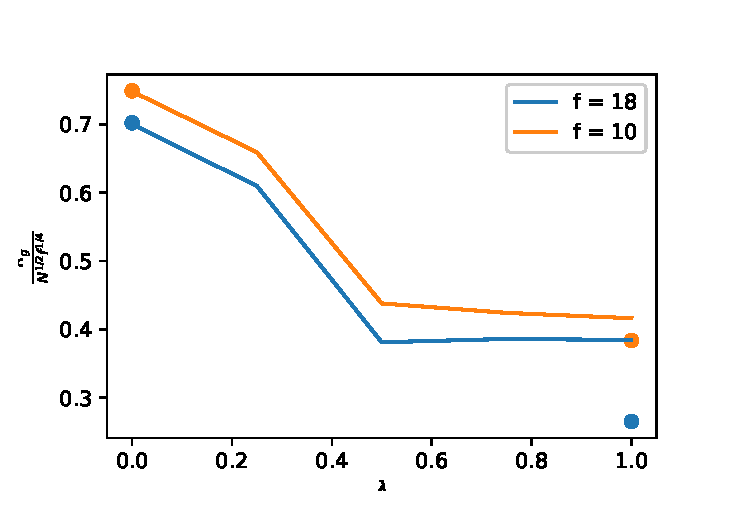
\includegraphics{figures/test_failed.eps}
    \caption{A not solved Bug. Normalized $R_g$, with $\lambda$. We expect around $\lambda = 0.48$. Curves collapse on eachother as shown by Huissman \textit{et al.}, and we should not see this differences with the scatter points, which are for the a normal Lennard-Jones potential implemented in Lammps.}
    \label{fig:enter-label}
\end{figure}